\documentclass[11pt,titlepage]{article}

\usepackage{graphicx}
\usepackage{color}
\usepackage{fancyvrb}
\usepackage{alltt}
\usepackage{amsmath}

\oddsidemargin 0.25in
\textwidth 6.0in
\topmargin -0.25in
\textheight 8.5in

\newenvironment{outdent}%
{\begin{list}{}%
{\listparindent=-1.5em\itemindent=\listparindent\leftmargin=1.5em}%
\item[]}%
{\end{list}}

\title{\bf Subdomain ADCIRC v.50 \\[3pt] User Guide}

\author{{\bf Technical Report CE-308-13} \\[60pt]
Developed by \\
Alper Altuntas and Jason Simon \\[40pt]
Under the direction of \\
John Baugh \\[40pt]
Department of \\
Civil, Construction, and Environmental Engineering \\
North Carolina State University \\
Raleigh, NC 27695 \\[50pt]}

\begin{document}

\pagenumbering{roman}
\maketitle
\tableofcontents
\setcounter{page}{2}

\newpage

\pagenumbering{arabic}

\section{Introduction}

ADCIRC is a computational hydrodynamic model widely used by scientists
and engineers to assess the effects of hurricane storm surge on
coastal areas. Extensive evaluation of storm surge often leads to the
consideration of multiple flooding scenarios that require substantial
computation times. Subdomain modeling is an approach to reduce the
total runtime of a series of hurricane storm surge simulations on a
smaller grid, a \emph{subdomain}, extracted from the original grid. By
enforcing the boundary conditions obtained from a full run, multiple
simulations on a subdomain with various local changes can be performed
in much less time.

% 2 Definitions
\section{Definitions}

This section provides definitions of the terms used in this
manual. The complete list of definitions of the parameters, input
files, and output files used in subdomain modeling is provided in
Appendices A.1 and A.2.

\begin{description}

\item[Full domain] a large geographical area usually requiring
  substantial computation times. A full domain run, performed once,
  provides the boundary conditions for a subdomain.

\item[Subdomain] a geographical area of interest within the full
  domain. Multiple subdomain runs with various local changes can be
  performed using the boundary conditions obtained from a full domain
  run.

\item[A subdomain modeling run] a subdomain run or a full domain run
  performed to provide the boundary conditions of a subdomain run.

\item[Subdomain modeling control file] an input file required for both
  full domain and subdomain runs. An ADCIRC subdomain modeling run
  first checks whether a subdomain control file exists in the domain
  directory. If the file exists, subdomain modeling is activated and
  the parameters of subdomain modeling are read from the input
  files. If the file does not exist, ADCIRC performs the simulation as
  usual.

\item[Shape file] a file specifying the location and size of a
  subdomain grid within the original full domain grid.

\item[Subdomain modeling input files] the collection of files used to
  configure both full domain and subdomain runs. For a subdomain run,
  input files consist of a shape file, a control file and a boundary
  conditions file. For a full domain run, the only input file is a
  subdomain modeling control file.

\end{description}

\section{Python Scripts}

Subdomain modeling Python scripts (\verb+gensub.py+,
\verb+genfull.py+, \verb+genbcs.py+) allow users to extract the
information from full domain input files and output files, and
generate subdomain input files including a nodal attributes file, grid
and boundary information file, subdomain control file, and boundary
conditions file. Users provide only the parameters that configure the subdomain
modeling approach and the locations of the subdomain and full domain
directories. 

\subsection{\texttt{gensub.py}}

\verb+gensub.py+ is used to create subdomain input files. This script
reads the subdomain shape file and full domain input files, and creates
the following input files in the subdomain directory:

\begin{itemize}
\item subdomain control file: \verb+[subdomain dir]/fort.015+ 
\item subdomain nodal attributes file: \verb+[subdomain dir]/fort.13+
\item subdomain grid information file: \verb+[subdomain dir]/fort.14+
\item subdomain mapping files: \verb+[subdomain dir]/py.14*+
\end{itemize}

\subsection{\texttt{genfull.py}}

\verb+genfull.py+ is used to create the full domain control file. This
script reads in the subdomain grid information file and mapping files,
and creates the control file in full domain directory:

\begin{itemize}
\item full domain control file: \verb+[fulldomain dir]/fort.015+ 
\end{itemize}

\subsection{\texttt{genbcs.py}}

\verb+genbcs.py+ is used to generate the boundary conditions file for
a subdomain grid. This script reads in full domain output files, and
creates the boundary conditions file in the subdomain directory:

\begin{itemize}
\item subdomain boundary conditions file: \verb+[subdomain dir]/fort.019+
\end{itemize}

\section{Overview of the Approach}

The construction of a subdomain model in ADCIRC consists of four main
steps. First, subdomain grid input files and control files are
generated. Second, a full domain ADCIRC run is performed. Third,
subdomain boundary conditions file is generated using full domain
output files. Finally, subdomain ADCIRC run is performed.
Figure~\ref{f1} summarizes the main steps of the subdomain modeling
approach, and Table~\ref{t1} lists the required input files and
generated output files for each of the Python scripts.  The following
section describes each of these steps in detail, including the usage
of Python scripts.

\begin{figure}
\centerline{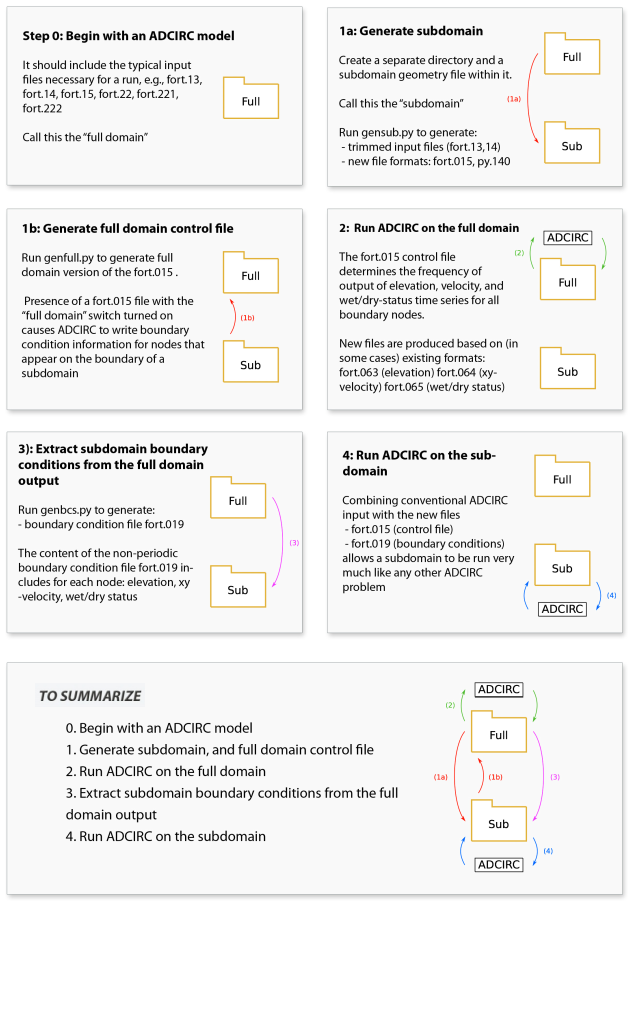
\includegraphics[width=0.95\textwidth]{workflows3.png}}
\caption{Summary of the work flow for subdomain modeling}
\label{f1}
\end{figure}

\begin{table}[htp]
\caption{Work Flow of Subdomain Modeling Approach} 
\label{t1}

{\renewcommand{\arraystretch}{1.3}
\begin{center}
\begin{tabular}[r]{l|c|r p{7.2cm}|}
	 	& \textbf{Grid}		& \multicolumn{2}{ l| }{\textbf{Description}} \\
\hline
\hline
\textbf{1a}	& \textbf{subdomain}	& \multicolumn{2}{ l| }{\textbf{Generate Subdomain}} \\
		&			& \emph{Python script:} & \verb+gensub.py+ \\
		&			& \emph{requires:} 	& \verb+[fulldomain]/fort.{13,14} +\\
		&			& 		 	& \verb+[subdomain]/shape.*14+\\
		&			& \emph{generates:} 	& \verb+[subdomain]/fort.{015,13,14} +\\
		&			& 		 	& \verb+[subdomain]/py.14* +\\
\hline
\textbf{1b}	& \textbf{fulldomain}	& \multicolumn{2}{ l| }{\textbf{Generate Full Domain Control File}} \\
		&			& \emph{Python script:} & \verb+genfull.py+ \\
		&			& \emph{requires:} 	& \verb+[subdomain]/{fort.14, py.14*} +\\
		&			& \emph{generates:} 	& \verb+[fulldomain]/{fort.015} +\\
\hline
\textbf{2}	& \textbf{fulldomain}	& \multicolumn{2}{ l| }{\textbf{Run ADCIRC on the full domain}} \\
		&			& \emph{Python script:} & \verb+-+ \\
		&			& \emph{requires:} 	& \verb+[fulldomain]/fort.{015,13,14...} +\\
		&			& \emph{generates:} 	& \verb+[fulldomain]/fort.065 +\\
\hline
\textbf{3}	& \textbf{fulldomain}	& \multicolumn{2}{ l| }{\textbf{Extract Subdomain Boundary Conditions}} \\
		&			& \emph{Python script:} & \verb+genbcs.py+ \\
		&			& \emph{requires:} 	& \verb+[fulldomain]/fort.065 +\\
		&			& \emph{generates:} 	& \verb+[subdomain]/fort.019 +\\
\hline
\textbf{4}	& \textbf{subdomain}	& \multicolumn{2}{ l| }{\textbf{Run ADCIRC on the subdomain}} \\
		&			& \emph{Python script:} & \verb+-+ \\
		&			& \emph{requires:} 	& \verb+[fulldomain]/fort.{015,019,13,14...} +\\
\hline

\end{tabular}
\end{center}}
\end{table}

\section{Detailed Instructions}

\subsection{Generate Subdomain}

First, create an empty subdomain directory. The Python script
\verb+gensub.py+ requires a shape file to extract the subdomain grid
from a full domain grid. Create the shape file using a text editor. A
shape file contains the coordinates and the size of a subdomain. Two
types of subdomain can be extracted from a full domain: circular and
elliptical. For a circular subdomain, name the shape file
``\verb+shape.c14+'', and for an elliptical subdomain, name the shape
file ``\verb+shape.e14+''.

\setlength\fboxsep{6pt}

The format of a shape file for a circular subdomain
(\verb+shape.c14+) consists of two lines: the coordinates of the
center of the subdomain and the radius.

\vspace{5pt}
\noindent
\mbox{}\hspace{30pt}\verb+shape.c14+\\[3pt]
\mbox{}\hspace{30pt}\fbox{
\begin{minipage}[t]{1in}
$x$ \ $y$ \\
$r$
\end{minipage}}
\vspace{11pt}

The format of a shape file for an elliptical subdomain
(\verb+shape.e14+) consists of three lines: the coordinates of the
first focal point, the coordinates of the second focal point, and the
width of the ellipse.

\vspace{5pt}
\noindent
\mbox{}\hspace{30pt}\verb+shape.e14+\\[3pt]
\mbox{}\hspace{30pt}\fbox{
\begin{minipage}[t]{1in}
$x_1$ \ $y_1$ \\
$x_2$ \ $y_2$ \\
$w$
\end{minipage}}
\vspace{11pt}

Once the shape file is saved in the subdomain directory, use the
Python script \verb+gensub.py+ to create subdomain input files:
\verb+fort.015+, \verb+fort.14+. If the full domain has a nodal
attributes file (\verb+fort.13+); the script can also generate a
\verb+fort.13+ file for the subdomain. The usage of
\verb+gensub.py+ is as follows:\footnote{The shape flag is 0 for
elliptical subdomains and 1 for circular subdomains.}

\begin{itemize}
\item To generate both \verb+fort.14+ and \verb+fort.13+ files:

\verb+$ python gensub.py [full fort.14] [shape flag] [new fort.14] +\\
\verb+                   [full fort.13] [new fort.13]+

\item To generate just a \verb+fort.14+ file:

\verb+$ python gensub.py [full fort.14] [shape flag] [new fort.14] +
\end{itemize}

\subsubsection*{\emph{Generate} \texttt{fort.15} \emph{file}}

The subdomain model parameter and periodic boundary condition file
(\verb+fort.15+) should be generated by the user. Copy the full domain
\verb+fort.15+ file to the subdomain directory. Modify the copied
\verb+fort.15+ file to ensure that the file is compatible with the
subdomain run. Required changes to a subdomain \verb+fort.15+ include:

\begin{itemize}
\item If the boundary conditions are not recorded at every timestep,
  slightly reduce \texttt{RNDAY} (e.g., by 0.5\%) to ensure that
  the boundary conditions file obtained from the full domain output
  files contains enough data to force the boundaries of the subdomain
  throughout the simulation.
\item Set \texttt{NBFR} (total number of forcing frequencies) to 0.
\item Remove lines that define periodic forcing frequencies. Since the
  boundaries of the subdomain are forced using a boundary conditions
  file, periodic forcing is not necessary.
\item Remove coordinates of any recording stations that are outside of
  the subdomain grid.
\item Update the number of recording stations.
\end{itemize}


\subsubsection*{\emph{Generate Meteorological Files}}

If the full domain has any meteorological
forcing files (e.g., \verb+fort.22+, \verb+fort.221+, \verb+fort.222+,
and so on) that define wind velocity and atmospheric pressure on 
rectangular (lat/lon) grid(s) , symbolically link these files in the 
subdomain directory. Meteorological files that define wind velocity
and atmospheric pressure at each grid node are required to be 
scaled by the user.


\subsubsection*{\emph{Generate full domain control file}}

The only subdomain modeling input file for a full domain run is the
control file, \verb+fort.015+.\footnote{If the control file does not
exist in the full domain directory, the ADCIRC run is performed as
usual, i.e., additional output files used to extract the boundary
conditions of a subdomain will not be generated.} The Python script
\verb+genfull.py+ is used to create the control file of a full domain
run. This script asks the user to input subdomain modeling parameter
\texttt{NSPOOLGS}
and directories\footnote{Directory paths passed to Python scripts as
arguments must end with a forward slash (\texttt{/}).} of the full
domain and subdomain runs.

The subdomain modeling approach in ADCIRC introduces a new output file
based on existing formats: \verb+fort.065+.
The sampling rate and reported nodes in this file is determined by
the user. The Python script \verb+genfull.py+ allows users to specify
the boundary nodes of the subdomains as the output nodes. Having an additional
set of output files allows ADCIRC to report the data of the boundary
nodes of a subdomain at a greater frequency while using less disk
space. There are two options for creating a \verb+fort.015+ file using
\verb+genfull.py+:

\begin{enumerate}
\item Assign the boundary nodes of previously created subdomains as
  output nodes. This option requires much less disk space, but it only 
  provides the output data for subdomain grids
  generated prior to the full domain run. Boundary node numbers of
  subdomains are automatically mapped to full domain node numbers and
  recorded in the \verb+fort.015+ file in the full domain
  directory. Any number of subdomains may be specified.

\item Assign all the full domain nodes as output nodes. This option may
  lead to excessively large output files, especially when the
  recording frequency is high. However, the availability of data for
  each node means that subdomains can later be generated anywhere in
  the full domain, providing greater flexibility.

\end{enumerate}

 The script first asks user to type in the parameter \texttt{NSPOOLGS}, the number of timesteps at which information is written to the new output file \texttt{fort.065}. Then, user is asked if predefined subdomain(s) will be provided. By entering ``\texttt{n}'', users can configure full domain run to record boundary conditions for every node in the full domain grid. If user types in ``\texttt{y}'', the script then asks for the subdomain directories in succession. Once the user enters all the directories, the generation of full domain control file can be finalized by entering ``\texttt{done}''.

  Usage:

  \verb+   $ python genfull.py [FullDomain Path]+

\subsection{Run ADCIRC on Full Domain}

Perform the full domain ADCIRC run to obtain the new set of output
files which are used to produce the boundary conditions of the
subdomain. Note that the subdomain modeling approach in ADCIRC is
activated only if the control file \verb+fort.015+ exists in the
working directory. Both serial and parallel ADCIRC can be used to
perform a full domain run.

\subsection{Extract Subdomain Boundary Conditions}

The boundary conditions file of a subdomain is generated using
\verb+genbcs.py+. This script reads the \verb+fort.065+ file of the 
full domain, and
produces a boundary conditions file, \verb+fort.019+, containing time
varying elevations, velocities, and wet/dry flags of boundary nodes,
inside the subdomain directory. The sampling rate of this file, called
\texttt{sbtiminc}, is determined by the
user.\footnote{\texttt{sbtiminc} must be a multiple of
\texttt{NSPOOLGS}, the number of time steps at which information is
written to full domain output files.}  The type of the full domain
run (serial or parallel) must be specified by the user.

  Usage:

  \verb+   $ python genfull.py [FullDomain Path][Subdomain Path][NOUTGS][sbtiminc]+

\mbox{}

Depending on the size of the grid and the sampling rate, producing the
boundary conditions using \verb+genbcs.py+ may take some time.

\subsection{Run ADCIRC on Subdomain}

The final step of subdomain modeling approach is to run ADCIRC on the
subdomain. Multiple ADCIRC runs with various local changes to the
subdomain model can be performed using the same boundary conditions
file, so long as changes in the hydrodynamics do not propogate out to
the subdomain boundaries.

\section{Example Usage on the Quarter Annular Test Case}

In this section, the subdomain modeling approach is applied to the
quarter annular test case, a simple example problem available from the
ADCIRC Development Group. The quarter annular grid shown in
Figure~\ref{f2} consists of 63 nodes and 96 triangular elements. The
outside arc is an open ocean boundary subject to tidal forces, and the
remaining sides are closed land boundaries.

\begin{figure}[ht]
\centerline{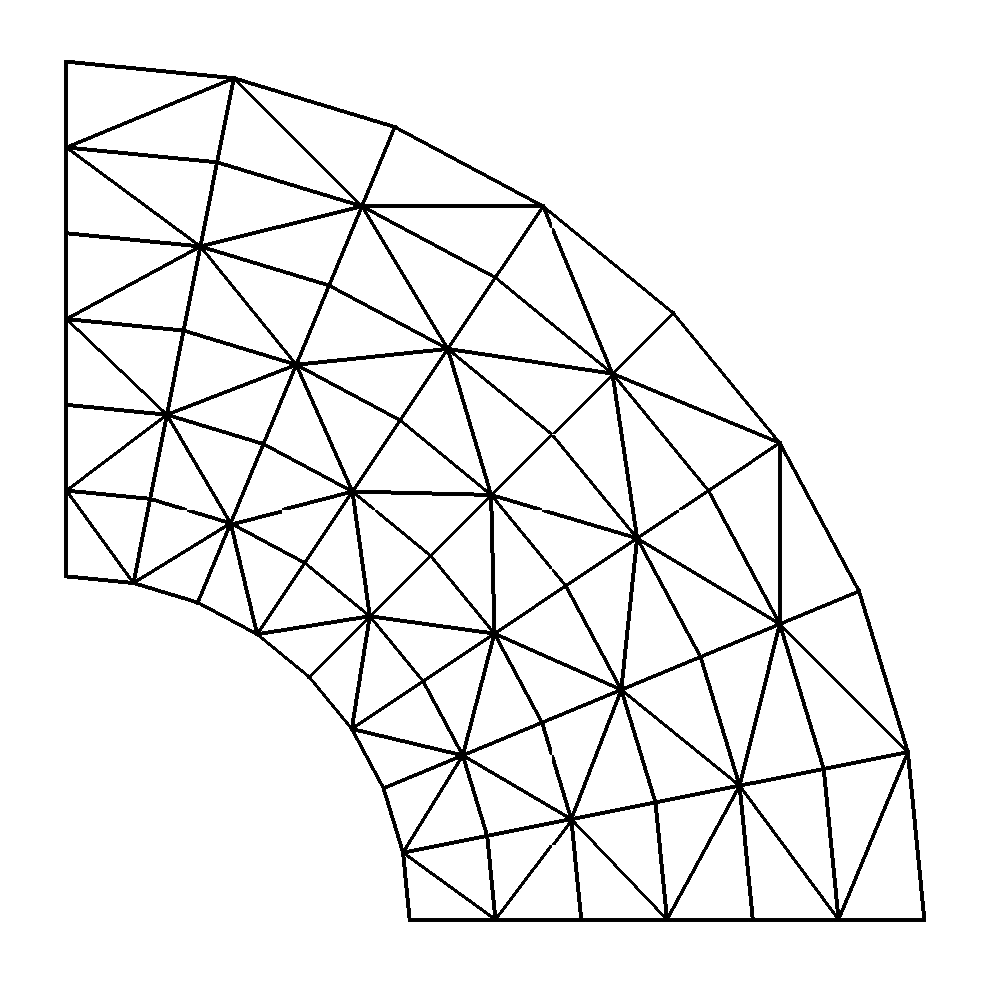
\includegraphics[width=5cm]{qatc.png}}
\caption{Quarter Annular Test Grid}
\label{f2}
\end{figure}

Using subdomain modeling Python scripts, an elliptical subdomain grid
consisting of 16 nodes and 18 elements is extracted from the original
quarter annular grid, as shown in Figure~\ref{f3}. Boundary conditions
are obtained from the original full run, and are then used for the
elliptical subdomain. The steps of the approach are described below.

\begin{figure}[ht]
\centerline{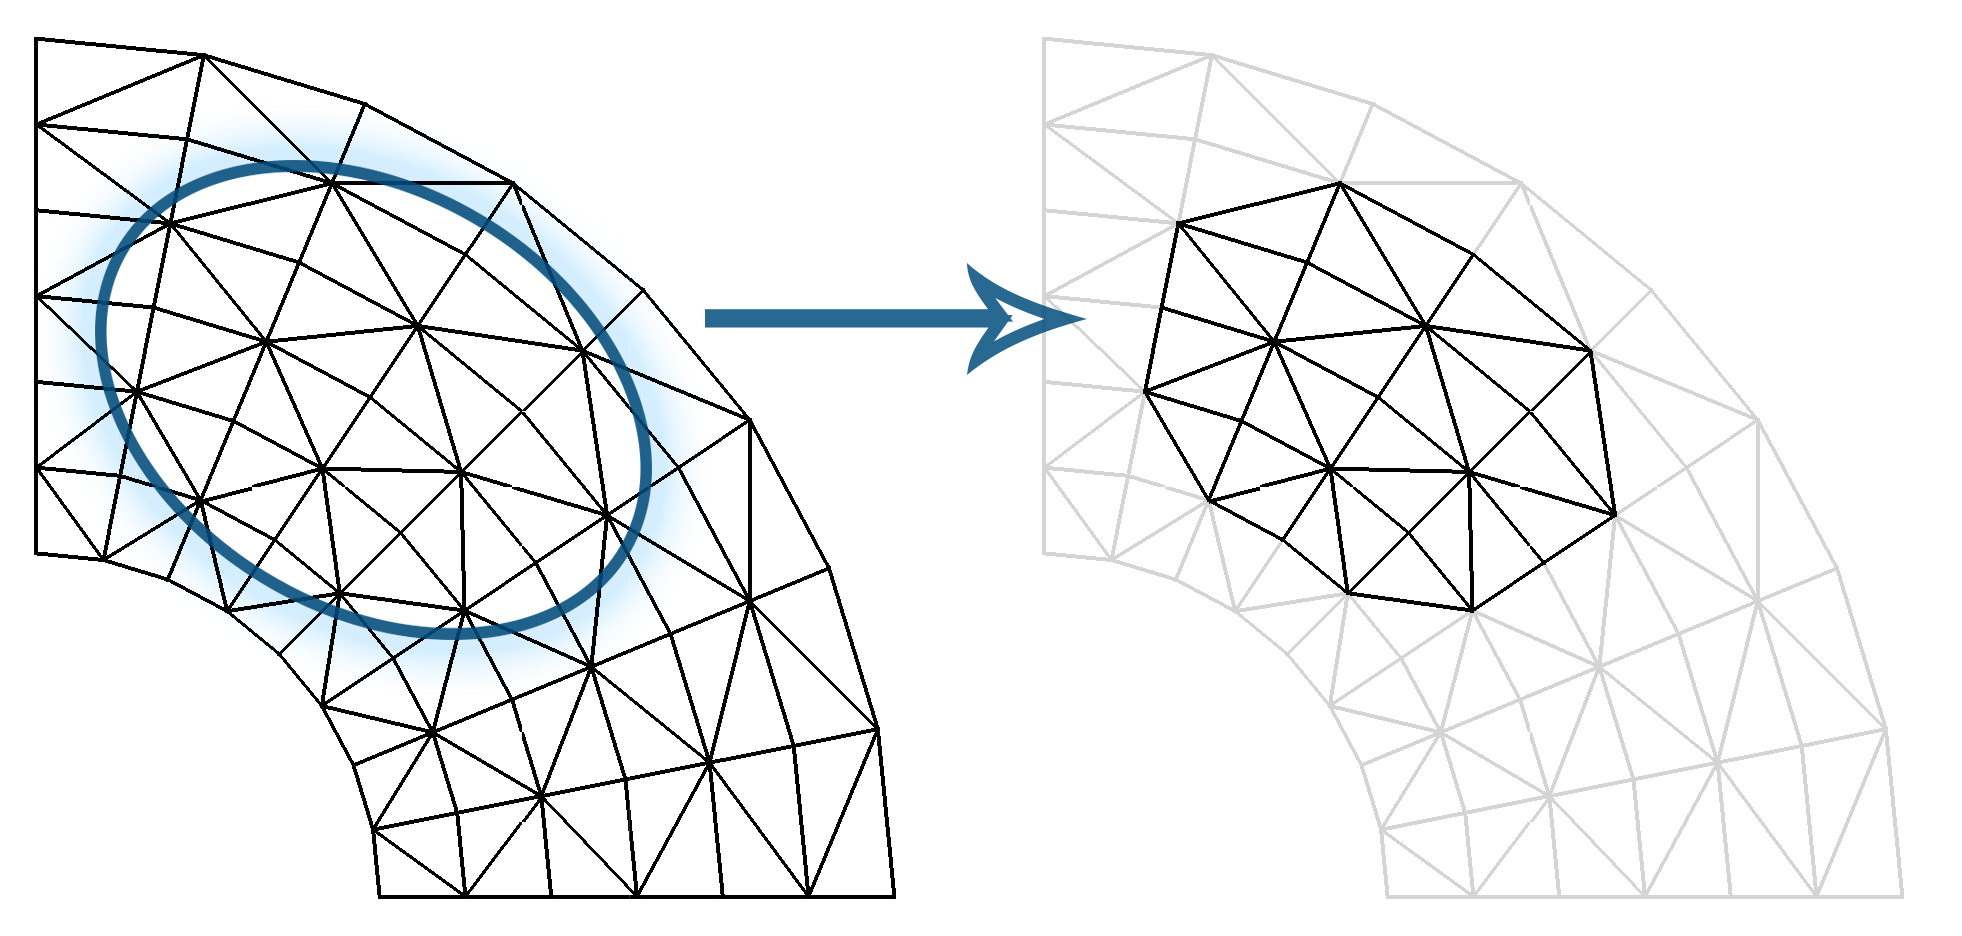
\includegraphics[width=11cm]{carveOut.png}}
\caption{Elliptical Subdomain Grid}
\label{f3}
\end{figure}

\subsection*{Generate Subdomain:}

\begin{enumerate}
\item Create an empty subdomain directory.
\item Create the shape file using a text editor, and save it in the
  subdomain directory.

\vspace{5pt}
\noindent
\mbox{}\hspace{30pt}\verb+shape.e14+\\[3pt]
\mbox{}\hspace{30pt}\fbox{
\begin{minipage}[t]{2in}
\texttt{40824.6 98559.5}\\
\texttt{98559.5 40824.6}\\
\texttt{60000}
\end{minipage}}
\vspace{11pt}

\item Move to the subdomain directory, and run \verb+gensub.py+ to
  generate the subdomain input files \verb+fort.14+ and
  \verb+fort.015+.\footnote{Additionally, auxiliary mapping files
  \texttt{py.140} and \texttt{py.141} will be created.} Note that the 
  directory path of a
  \verb+fort.13+ file is not specified, since this example does not
  require a nodal attributes file.

\begin{verbatim}
$ python [script dir]/gensub.py [full.dir]/fort.14 0 fort.14

\end{verbatim}

\item Copy the full domain \verb+fort.15+ file to the subdomain
  directory, and modify it as follows\footnote{The resulting subdomain
  \texttt{fort.15} file is shown in Appendix A.4.}:

\begin{itemize}
\item Set \verb+NBFR+ to 0.
\item Remove the lines that are related to periodic forcing
  frequencies.\footnote{In this example, 12 lines after the line with
  \texttt{NBFR}.}
\item Remove the coordinates of elevation and velocity recording
  stations.
\item Set number of elevation and velocity recording stations to 0.
\end{itemize}
Note that this example does not require any meteorological file.

\item Move to the full domain directory and run \verb+genfull.py+ to
  generate the full domain control file \verb+fort.015+. Although file
  sizes are of no concern in this small example, only the boundary
  nodes of the subdomain are written to the full domain
  \verb+fort.015+ file to illustrate the approach. Note that directory
  paths passed to Python scripts as arguments must end with a forward
  slash (\texttt{/}) (e.g., \verb+/home/[user]/qa-subdomain/+).

\begin{verbatim}
$ python [script dir]/genfull.py ./

Enter the parameter 'NSPOOLGS' (the freq. of forcing in no. of timesteps): 
1
	 Reading fort.14 at ./
Specify predetermined subdomains? (y or n) 
y
Enter the directory of the subdomain: (Type 'done' to end)
../qa-sub/
	 Reading boundary information of ../qa-sub/
	 Reading fort.14 at ../qa-sub/
	 Reading py.140 at  ../qa-sub/
	 Subdomain info at ../qa-sub/ is added to the full domain control file.
Enter the directory of the subdomain: (Type 'done' to end)
done
 fort.015 file for the full run is ready.
\end{verbatim}

 The script asks user to type in the parameter \texttt{NSPOOLGS}. For this example problem, type ``\texttt{1}'' and press \texttt{enter}. By setting \texttt{NSPOOLGS} to 1, it is ensured that the boundary information for the subdomain run will be recorded at every timestep. The script then asks user if predefined subdomain(s) will be provided. Since a subdomain is created prior to ADCIRC full domain run, type in ``\texttt{y}'', and press \texttt{enter}. The script then asks users to type in the subdomain directories. Enter the directory to the subdomain grid. Enter ``\texttt{done}'' to finalize the generation of full domain control file.


\end{enumerate}


\subsection*{Run ADCIRC on Full Domain: }

Perform the full domain ADCIRC run, either in serial or in parallel.


\subsection*{Extract Subdomain Boundary Conditions:}
\begin{enumerate}
\item Move to the subdomain directory.
\item Generate the \verb+fort.019+ boundary conditions file for the
  subdomain run using \verb+genbcs.py+.
\begin{verbatim}
$ python [script dir]/genbcs.py [full dir] [sub dir] 1 1

Enter the type of the full run (p for parallel, s for serial):
s
	 Reading fort.14 at ../qa/
	 Reading fort.14 at ./
	 Reading py.140 at  ./
\end{verbatim}

The script as users if the full domain run was performed using serial ADCIRC or parallel ADCIRC. Type in \verb+s+ or \verb+p+ accordingly.

\end{enumerate}


\subsection*{Run ADCIRC on Subdomain:}

Perform the subdomain ADCIRC run, either in serial or in parallel.



\subsubsection*{\emph{Maximum elevation difference}}

Maximum elevations files of both runs are compared, and it is 
observed that the largest difference between the full domain
run and the enforced subdomain run at a node is $
2 \times 10^{-7}$ meters.






\appendix

\newpage

\section{Appendix}

\subsection{Subdomain Modeling Parameters}

\begin{description}

\item[NOUTGS:] Subdomain modeling flag for a full domain run. 
By setting this parameter to 1 in the full domain control file, the 
required  subdomain boundary conditions for Type-1 are 
recorded, and by setting this parameter to 2, the required subdomain 
boundary conditions for Type-2 are recorded. 
Note: Type-2 runs are for test purposes only.

\item[NSPOOLGS:] The number of timesteps at which information is 
written to the new set of output files; fort.06*.

\item[enforceBN:] Subdomain modeling flag for a subdomain run.
Type-1 is activated by setting this parameter to 1 in 
the subdomain control file, and Type-2 is activated by 
setting this parameter to 2. Note that the required boundary 
conditions file(s) need to exist in the subdomain directory.

\item[ncbnr:] The number of outer boundary nodes of Type-1 
subdomain grids to be recorded during a full run. 

\item[cbnr:] Array of nodes containing the outer boundary nodes
of Type-1 subdomain grids to be recorded during a full run.

\item[ncbn:] The number of outer boundary nodes of a Type-1 subdomain.

\item[eta2(n):] Forced elevation at node n.

\item[etas(n):] Forced elevation change at node n.

\item[uu2(n):] Forced x velocity at node n.

\item[vv2(n):] Forced y velocity at node n.

\item[nodecode(n):] Forced wet/dry flag at node n.

\end{description}

\subsection{Subdomain Modeling File Formats}

\subsubsection{\texttt{fort.015} - Model control parameters}

\begin{alltt}
NOUTGS
NSPOOLGS
enforceBN
ncbnr
\emph{ for cnode in cbnr:}
\quad cnode


\end{alltt}


\subsubsection{\texttt{fort.019} - Subdomain boundary conditions file (enforceBN=1) }

\begin{alltt}
header
nspoolgs, ncbnr, #timesteps
\emph{for n in cbnr:}
\quad n
\emph{for it in #timesteps:}
\quad it
\quad \emph{for n in cbn:}
\quad \quad n, eta2(n), uu2(n)
\quad \quad vv2(n), nodecode(n)

\end{alltt}




\subsubsection{\texttt{fort.065} - Full domain output file (noutgs=1) }

\begin{alltt}
header
nspoolgs, ncbnr, #timesteps
\emph{for it in #timesteps:}
\quad it
\quad \emph{for n in cbnr:}
\quad \quad n, eta2(n), uu2(n)
\quad \quad vv2(n), nodecode(n)

\end{alltt}



\subsection{Modified fort.15 file for the elliptical QATC subdomain}

{\small
\begin{verbatim}
 QUARTER ANNULAR TEST EXAMPLE 1      
 ADCIRC V41.03                       
 0                                   ! NFOVER 
 0                                   ! NABOUT 
 1                                   ! NSCREEN 
 0                                   ! IHOT 
 1                                   ! ICS
 0                                   ! IM 
 1                                   ! NOLIBF 
 1                                   ! NOLIFA
 1                                   ! NOLICA 
 1                                   ! NOLICAT 
 0                                   ! NWP 
 0                                   ! NCOR
 0                                   ! NTIP
 0                                   ! NWS
 1                                   ! NRAMP
 9.81                                ! G 
 0.005                               ! TAU0 
 174.656                             ! DT 
 0.00                                ! STATIM
 0.00                                ! REFTIM 
 5                                 ! RNDAY 
 2.0                                 ! DRAMP
 0.35 0.30 0.35                      ! TIME WEIGHTING FACTORS FOR THE GWCE EQUATION
 1.0                                 ! H0 
 0.0 0.0                             ! SLAM0,SFEA0 
 0.0025                              ! FFACTOR 
 0.0                                 ! ESL
 0.0                                 ! CORI 
 0                                   ! NTIF 
 0                                   ! NBFR 
 110.0                               ! ANGINN 
 1 0.0 5.0  3                        ! NOUTE,TOUTSE,TOUTFE,NSPOOLE
 0                                   ! TOTAL NUMBER OF ELEVATION RECORDING STATIONS
 1 0.0 5.0  3                        ! NOUTV,TOUTSV,TOUTFV,NSPOOLV
 0                                   ! TOTAL NUMBER OF VELOCITY RECORDING STATIONS
 1 0.0 5.0 1                         ! NOUTGE,TOUTSGE,TOUTFGE,NSPOOLGE 
 1 0.0 5.0 1                         ! NOUTGV,TOUTSGV,TOUTFGV,NSPOOLGV
 1                                   ! NHARFR
 M2                                  ! HAFNAM(I)
 0.0001405257 1.0 0.0                ! HAFREQ(I=1),HAFF(I=1),HAFACE(I=1)
 4.00  5.00  1  0.0                  ! THAS,THAF,NHAINC,FMV 
 1 1 1 1                             ! NHASE,NHASV,NHAGE,NHAGV 
 1 512                               ! NHSTAR,NHSINC 
 1  0  1.E-5  25                     ! ITITER, ISLDIA, CONVCR, ITMAX
\end{verbatim}}

\newpage

\section{Acknowledgments}

This material is based upon work supported by the Coastal Hazards
Center of Excellence, a US Department of Homeland Security Science and
Technology Center of Excellence under Award Number: 2008-ST-061-ND
0001, and a Department of Homeland Security HS-STEM Career Development
Grant.

The views and conclusions contained in this document are those of the
authors and should not be interpreted as necessarily representing the
official policies, either expressed or implied, of the US Department
of Homeland Security.

The authors wish to thank Dr.~Rick Luettich and Dr.~Brian Blanton for
their assistance with ADCIRC and for providing base grids and input
files.

\section{List of Publications and Talks}

\begin{outdent}
Altuntas, A. (2012). ``Downscaling storm surge models for engineering
applications.'' M.S.~Thesis, NC State University, Raleigh, NC, July.\\
{\small \verb![http://www.lib.ncsu.edu/resolver/1840.16/8035]!}

Baugh, J. W. (2012). ``Subdomain modeling.'' 2012 ADCIRC Workshop,
NOAA in Silver Spring, MD, April 23--24.

Baugh, J. W., Rutledge, J., Altuntas, A., and Dyer, T. (2012).
``Downscaling storm surge models for engineering applications.'' Tenth
International Conference on Hydroscience \& Engineering (ICHE),
Orlando, FL, November 4--7.

Baugh, J. W., and Simon, J. S. (2011). ``Localized storm surge
modeling for engineering analysis and design.'' ECM 12: Twelfth
International Conference on Estuarine and Coastal Modeling,
St. Augustine, FL, November 7--9.

Simon, J. S. (2011). ``A computational approach for local storm
surge modeling.''  M.S.~Thesis, North Carolina State University,
Raleigh, NC, June.\\
{\small \verb![http://www.lib.ncsu.edu/resolver/1840.16/7179]!}

Simon, J. S., and Baugh, J. W. (2011). ``Localized modeling of storm
surge effects on civil infrastructure using nested meshes.'' WRRI
Annual Conference, Raleigh, NC, March 22--23.
\end{outdent}



\end{document}